\chapter{Molecular motor tug-of-war can achieve viral capsid disassembly}
\label{ch:TugOfWar-chapter}

\dictum[Sarah Kay]{%
  Is there a word for the moment you win tug-of-war? When the weight gives, and all that extra rope comes hurtling towards you, how even though you've won, you still end up with muddy knees and burns on your hands? Is there a word for that? I wish there was.}%
\vskip 1em

\section{Introduction}

\section{Effective forces on nanomolecular scales}
In classical mechanics an object moving in fluid is affected by forces: weight (directed down), buoyant force (directed up), drag force (directed opposite the direction of movement). During capsid disassembly there are also forces exerted by molecular motors and restoring forces of bonds between M1.

\begin{center}
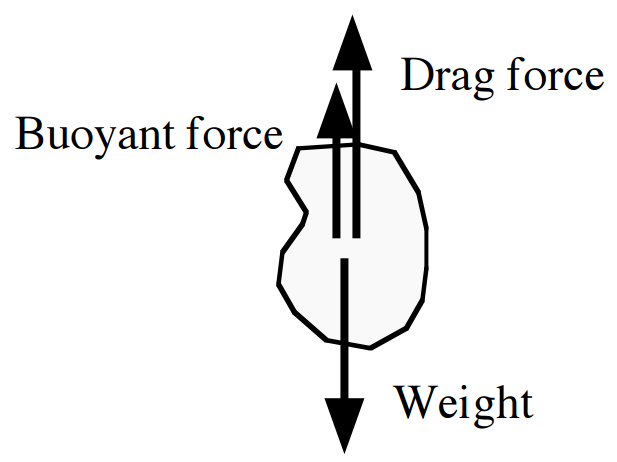
\includegraphics[width=0.5\textwidth]{D_chapters/1_TugOfWar/Sedimentation.PNG}
\captionof{figure}{Forces affecting object during sedimentation in fluid.}
\end{center}

The Reynolds number is the ratio of inertial forces to viscous forces within a fluid which is subjected to relative internal movement due to different fluid velocities. In systems with low Reynolds numbers it's sometimes possible to omit inertial forces as fluid dynamic play a much more important role \cite{purcell1977life}.

Let's estimate sedimentation forces and mechanical forces involved in capsid disassembly, to determine their relevancy to mathematical modelling.

\subsection{Reynolds number}

Reynolds number is defined as

\begin{equation}
Re = \frac{\text{inertial forces}}{\text{viscous forces}} =\frac{av\rho}{\eta} = \frac{av}{\nu}
\end{equation}

where $a$ is a characteristic size of the moving object, $v$ is its velocity relative to fluid, $\rho$ is fluid density, $\eta$ is fluid viscosity and $\nu$ is kinematic viscosity.

\begin{center}
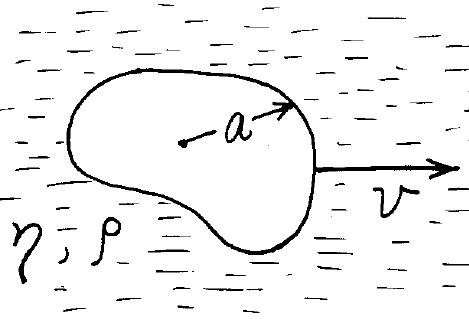
\includegraphics[width=0.5\textwidth]{D_chapters/1_TugOfWar/Reynolds_number.PNG}
\captionof{figure}{Object of characteristic size $a$ moving with speed $v$ in fluid with density $\rho$ and viscosity $\eta$.}
\end{center}

Let's calculate Reynolds number for influenza A capsid protein M1.

M1 characteristic size $a = 4 \text{ nm} = 4 \cdot 10^{-7} \text{ cm}$ \cite{shtykova2013structural}.

During calculation individual velocities of the nodes typically are in the range of $10^{-13}$-$10^{-5} \text{ m/s}$. Motor forward velocities are around $10^{-6} \text{ m/s}$ \cite{muller2008tug}. Let's assume for this calculation that $v = 10^{-6} \text{ m/s} = 10^{-4} \text{ cm/s}$.

Average density of the cytoplasm (horn cells in rats, only available data?) is about $\rho = 0.3 \text{ pg}/\SI{}{\micro\meter}^3 = 0.3 \text{ g}/\text{cm}^3$ \cite{hartmann1967cytoplasmic}. Alternatively (\textit{E. coli}) $\rho = 1.1 \text{ g}/\text{cm}^3$ \cite{loferer1998determination}.

Relative viscosity of cytoplasm (cytoplasm versus water) determined by time-resolved microfluorimetry \cite{swaminathan1997photobleaching} is

\begin{equation}
\frac{\eta_\text{cytoplasm}}{\eta_\text{water}} = 1.5,
\end{equation}

and determined by photobleaching recovery of green fluorescent protein \cite{swaminathan1997photobleaching} is 

\begin{equation}
\frac{\eta_\text{cytoplasm}}{\eta_\text{water} }= 3.2.
\end{equation}

Water viscosity is $\eta_\text{water} = 8.9 \cdot 10^{-3} \text{ dyn} \cdot \text{s}/\text{cm}^2 = 8.9 \cdot 10^{-3} \text{ g}/\text{cm} \cdot \text{s} $ at \SI{25}{\degreeCelsius} \cite{IAPWS2008}. So $\eta_\text{cytoplasm} = 3.2 \cdot 8.9 \cdot 10^{-3} \text{ g}/(\text{cm} \cdot \text{s}) = 28.5 \cdot 10^{-3} \text{ g}/(\text{cm} \cdot \text{s})$.

Thus, Reynolds number is

\begin{equation}
Re = \frac{av\rho}{\eta} = \frac{4 \cdot 10^{-7} \text{ cm} \cdot 10^{-4} \text{ cm/s} \cdot 0.3 \text{ g}/\text{cm}^3}{28.5 \cdot 10^{-3} \text{ g}/(\text{cm} \cdot \text{s})} = 4.2 \cdot 10^{-10}
\end{equation}

This value is extremely small - for comparison, the Reynolds number for a bacteria moving in the medium is (?)

\subsection{Weight}

\begin{equation}
F_{\text{weight}} = mg,
\end{equation}

where $m$ is object mass and $g$ is gravitational acceleration.

The mass of M1 capsid protein is $m_{\text{M1}} = 28 \text{ kDa} = 28 \cdot 1000 \cdot 1.66 \cdot 10^{-27} \text{ kg} = 46.5 \cdot 10^{-24} \text{ kg}$. \cite{shtykova2013structural}

Then the force is

\begin{equation}
F_{\text{weight}} = m_{M1}g = 46.5 \cdot 10^{-24} \text{ kg} \cdot 9.8 \text{ m}/\text{s}^2 = 4.6 \cdot 10^{-22} \text{ N}
\end{equation}

\subsection{Buoyant force}

\begin{equation}
F_{\text{buoyant}} = \rho_FVg,
\end{equation}

where $\rho_F$ is density of the fluid, $V$ is the volume of the object and $g$ is gravitational acceleration.

Density of cytoplasm as previously established is $\rho = 0.3 \text{ g}/\text{cm}^3 = 3000 \text{ kg}/\text{m}^3$ \cite{hartmann1967cytoplasmic}

Dimensions of M1 protein are approximately $4.0 \times 4.0 \times 6.0 \text{ nm}$ \cite{shtykova2013structural}, so $V_{M1} = 96 \text{ nm}^3 = 9.6 \cdot 10^{-26} \text{ m}^3$

Then the force is

\begin{equation}
\begin{split}
F_{\text{buoyant}} = \rho_{\text{cytoplasm}}V_{M1}g =\\
3000 \text{ kg}/\text{m}^3 \cdot 9.6 \cdot 10^{-26} \text{ m}^3 \cdot 9.8 \text{ m}/\text{s}^2 =\\
2.8 \cdot 10^{-21} \text{ N}
\end{split}
\end{equation}

\subsection{Drag force}

Drag force exerted on spherical objects with very small Reynolds numbers (i.e. very small particles) in a viscous fluid is defined by Stokes' law:

\begin{equation}
F_{\text{drag}} = 6\pi\eta av,
\end{equation}

where $\eta$ is dynamic fluid viscosity, $a$ is the radius of the spherical object, $v$ is the flow velocity relative to the object.

As previously shown $\eta_{\text{cytoplasm}} = 28.5 \cdot 10^{-3} \text{ g}/(\text{cm} \cdot \text{s}) = 2.85 \cdot 10^{-4} \text{ kg}/(\text{m} \cdot \text{s})$ \cite{swaminathan1997photobleaching, IAPWS2008}.

M1 characteristic size $a = 4 \text{ nm} = 4 \cdot 10^{-9} \text{ m}$ \cite{shtykova2013structural}.

And velocities are in range $v = 10^{-6} \text{ m/s}$ \cite{muller2008tug}.

Then the force is

\begin{equation}
\begin{split}
F_{\text{drag}} = 6\pi\eta_{\text{cytoplasm}} av = \\
6 \cdot 3.14 \cdot 2.85 \cdot 10^{-4} \text{ kg}/(\text{m} \cdot \text{s}) \cdot 4 \cdot 10^{-9} \text{ m} \cdot 10^{-6} \text{ m/s} =\\
2.1 \cdot 10^{-17} \text{ N}.
\end{split}
\end{equation}

\begin{center}
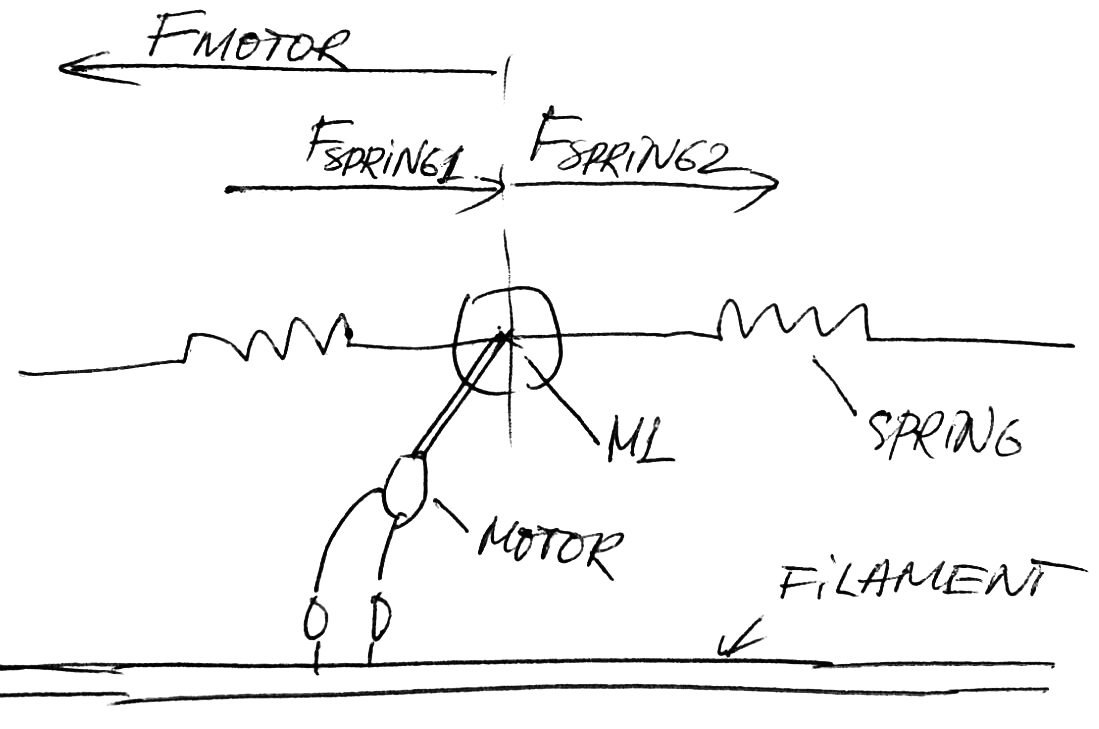
\includegraphics[width=0.5\textwidth]{D_chapters/1_TugOfWar/Capsid.jpg}
\captionof{figure}{Forces affecting M1 capsid protein during capsid disassembly.}
\end{center}

\subsection{Motor forces}

Stall forces of molecular motors are in orders of pN \cite{muller2008tug}, which leads to resulting tug-of-war forces to be of the same order $F_{\text{motor}} = 10^{-12} \text{ N}$.

\subsection{Spring forces}

In the simplest case spring forces can be calculated using Hooke's law:

\begin{equation}
F_{\text{Hooke}} = k_{\text{spring}}\Delta x.
\end{equation}

At pH of interest the bond spring constant is $k_{\text{spring}} = 2.1 \cdot 10^{-2} \text{ N}/\text{m}$ \cite{li2014ph}

The displacements in the calculation are of the order of the equilibrium length of the spring: $\Delta x = 4 \text{ nm} = 4 \cdot 10^{-9} \text{ m}$

Then the force is

\begin{equation}
\begin{split}
F_{\text{Hooke}} = k_{\text{spring}}\Delta x =\\
2.1 \cdot 10^{-2} \text{ N}/\text{m} \cdot 4 \cdot 10^{-9} \text{ m} = 8.4 \cdot 10^{-11} \text{ N}.
\end{split}
\end{equation}

In our representation of capsid disassembly instead of Hooke's law we're using Morse potential, because it explicitly includes the possibility of break:

\begin{equation}
V(\mathbf{r}) = D_{\text{e}} \big(1 - e^{- a(\mathbf{r - r_e})}\big)^2 = D_{\text{e}} \big(1 - e^{- a \Delta \mathbf{r}}\big)^2.
\end{equation}

Here $\mathbf{r}$ is the distance, $\mathbf{r_e}$ is the equilibrium bond distance, $D_{\text{e}}$ is the well depth,

\begin{equation}
a=\sqrt {\frac{k_{\text{e}}}{2D_{\text{e}}}},
\end{equation}

where $k_e$ is the force constant at the minimum of the well. $a$ controls the ``width'' of the potential (the smaller $a$ is, the larger the well).

The restoring force is

\begin{equation}
\mathbf{F}_\text{Morse} = - 2a D_{\text{e}}e^{- a |\Delta \mathbf{x}|}\big(1 - e^{- a |\Delta \mathbf{x}|}\big) \cdot \big(- \frac{\Delta \mathbf{x}}{|\Delta \mathbf{x}|}\big).
\end{equation}

For $D_{\text{e}} = 20 \text{kJ}$ (the energy of hydrogen bond \cite{mcnaught1997compendium}) and $k_{\text{e}} = k_{\text{spring}} = 2.1 \cdot 10^{-2} \text{ N}/\text{m}$

\begin{equation}
\begin{split}
a = \sqrt {\frac{2.1 \cdot 10^{-2} \text{ N}/\text{m}}{2 \cdot 2 \cdot 10^{4} \text{J}}}\\
= \sqrt {\frac{2.1 \cdot 10^{-2} (\text{ kg} \cdot \text{m} \cdot \text{s}^-2)/\text{m}}{2 \cdot 2 \cdot 10^{4} (\text{ kg} \cdot \text{m}^2 \cdot \text{s}^-2)}} = 7.2 \text{ m}^{-1}
\end{split}
\end{equation}

\begin{equation}
e^{- a |\Delta \mathbf{x}|} = e^{- 7.2 \text{ m}^{-1} \cdot 4 \cdot 10^{-9} \text{ m}} = 1
\end{equation}

\begin{equation}
1 - e^{- a |\Delta \mathbf{x}|} = 1 - e^{- 7.2 \text{ m}^{-1} \cdot 4 \cdot 10^{-9} \text{ m}} = 2.9 \cdot 10^{-9}
\end{equation}

\begin{equation}
\begin{split}
F_\text{Morse} = 2aD_{\text{e}}e^{- a |\Delta \mathbf{x}|}\big(1 - e^{- a |\Delta \mathbf{x}|}\big) =\\
2 \cdot 7.2 \text{ m}^{-1} \cdot 2 \cdot 10^{4} \text{J} \cdot 1 \cdot 2.9 \cdot 10^{-9} = 8.4 \cdot 10^{-4} \text{ N}.
\end{split}
\end{equation}

On first calculation steps these forces are about $10^{-21} \text{ N}$ but reach up to $10^{-9} \text{ N}$ during the course of the calculation.

\subsection{Conclusion}

In our model we can only focus on spring and motor forces as sedimentation forces acting on the proteins are negligibly small.



\section{Methods}
The mass-spring mathematical model for capsid breakage represents a rectangular fragment of the capsid at the stage when it is exposed via the fusion pore and is interacting with host molecular motors, which pull it apart (Figure 2A).

Capsid M1 proteins (the masses) are arranged in a regular mesh approximately of the size of the fusion pore (see Table S1 for all parameter values). Edge nodes of the mesh are bound to the lipid bilayer of the viral envelope/endosome and inner nodes are exposed to the cytoplasm. Here, we used a 6x6 mesh with 4x4 inner capsid proteins. Each inner mass is computed as the sum of protein masses bound to a particular node. For example, a free capsid node would simply correspond to the M1 protein mass, while a node attached to a myosin motor would have a total mass equal to the sum of masses of M1 protein, HDAC6, Ub, and myosin. Each edge node mass is the average mass of the endosome divided by the number of edge nodes.

The masses are connected to each other with elastic bonds, which we represent as a Morse potential that can explicitly include effects of bond breaking. Specifically, the Morse potential is

$V_{Morse} (r) = D_e (1 - \exp(-a(r - r_e)^2))$ , with  $a = \sqrt{\frac{k^2_e}{D_e}}$,

which has two parameters: stiffness $k_e$ and dissociation energy $D_e$. In this model we use two sets of Morse parameters for inner and outer nodes.

Each of the inner nodes of the capsid is acted on by the elastic forces of the 4 springs connecting it to other nodes. We calculate the change in spring length between two nodes as

$\delta l = \sqrt{(\delta x)^2 + (\delta y)^2} - l_{equilibrium}$ ,
 
where $\delta x = x_{neighbor} - x_{current}$ and $\delta y = y_{neighbor} - y_{current}$ are the differences between the x and y coordinates of the neighbor node and the current node, and $l_{equilibrium}$ is the equilibrium spring length. The change in spring length $\delta l$ determines the force acting on the node, created by each particular spring. We compute the force as

$f_{Morse spring} = -2 a^{type} D^{type} \exp(-a^{type} \delta l) (1 - \exp(-a^{type} \delta l))$,
 
where $a^{type}$ and $D^{type}$ are the parameters of the Morse spring, depending on the spring’s type (inner nodes corresponding to capsid parameters and edge nodes to capsid with lipid bilayer cover).

We then compute the projections on the x and the y axis of the acceleration created by each of the spring forces as follows:

$a^{spring}_z = \frac{f_{Morse spring}}{m_{node}} (\frac{-\delta z}{(\delta x)^2 + (\delta y)^2})$ ,

where $m_{node}$ is the node’s mass and $z$ stands for either x or  y.

Finally, the ODE system for one node looks as follows

\begin{equation}
\frac{d}{dt}
\begin{pmatrix}
position x\\
position y\\
velocity x\\
velocity y\\
time
\end{pmatrix}
=
\begin{pmatrix}
velocity x\\
velocity y\\
a^{top}_x + a^{right}_x + a^{bottom}_x + a^{left}_x + \frac{f^{motor}_x}{m_{node}}\\
a^{top}_y + a^{right}_y + a^{bottom}_y + a^{left}_y + \frac{f^{motor}_y}{m_{node}}\\
1
\end{pmatrix}
\end{equation}

We model the cytoskeleton near the fusion pore by a single, randomly directed microtubule, and by a denser network of actin filaments with a nucleation point on one of the edge nodes. Molecular motors are directly or indirectly (which we do not distinguish in this model) connected to the exposed capsid M1 proteins and to the cytoskeleton, allowing them to exert forces on the capsid. Specifically, dynein motors can walk in a single direction along the microtubule, while myosin motors can walk along actin filaments in random directions away from the nucleation point. Dyneins can connect to any of the inner nodes, but they can only exert forces on the capsid if they fall within the microtubular area of effect, determined by its width (Figure 2A).
We compute the resulting forces through a tug-of-war model with experimentally determined motor characteristics \cite{gennerich2007force, muller2008tug, norstrom2010unconventional}, which we modified to represent dyneins, kinesins, and positive- and negative-direction myosins. Importantly, the model considers that the force exerted by each individual motor depends on all the other motors bound to the same cargo.
First, let us examine the one-dimensional case, where all the motors walk along the microtubule. Analogously to the two-motor scenario  \cite{gennerich2007force, muller2008tug, norstrom2010unconventional}, we write a force balance.

\begin{equation}
n_kf_k + n_{m+}f_{m+} = -n_df_d - n_{m-}f_{m-} = f_C(n_k, n_d, n_{m+}, n_{m-})
\end{equation}

where $n_k$, $n_d$, $n_{m+}$, $n_{m-}$ are motor numbers and $f_k$, $f_d$, $f_{m+}$, $f_{m-}$ are forces of kinesin, dynein, plus- and minus-end myosin motors, respectively. The cargo force is determined by the condition that all motors move with the same velocity $v_C$ , as given by

\begin{equation}
v_C(n_k, n_d, n_{m+}, n_{m-}) = v_k(f_k) = v_{m+}(f_{m+}) = - v_d(f_d) = - v_{m-}(f_{m-})
\end{equation}

With this definition follows for the left part of the force balance equation Eq. (0.1)

\begin{equation}
f_C(n_k, n_d, n_{m+}, n_{m-}) = n_kf_k + n_{m+}f_{m+} = n_kf_k\big(1 + \frac{n_{m+}f_{m+}}{n_kf_{k}}\big)
\end{equation},

which gives us an expression for the kinesin force:

\begin{equation}
f_k = \frac{f_C(n_k, n_d, n_{m+}, n_{m-})}{n_k\big(1 + \frac{n_{m+}f_{m+}}{n_kf_{k}}\big)}
\end{equation}.

Analogously, for the right part and the dynein force, we obtain:

\begin{equation}
f_d = -\frac{f_C(n_k, n_d, n_{m+}, n_{m-})}{n_d\big(1 + \frac{n_{m-}f_{m-}}{n_df_{d}}\big)}
\end{equation}.

For simplicity, we assume here that the ratio of motor forces moving in the same direction is proportionate to the ratio of their stall forces (indicated by subscript S):

\begin{equation}
\frac{f_{m+}}{f_k} \propto \frac{f_{Sm+}}{f_{Sk}}, 
\frac{f_{m-}}{f_d} \propto \frac{f_{Sm-}}{f_{Sd}}
\end{equation}

This allows us to write the expressions for kinesin and dynein forces as follows

\begin{equation}
f_k = \frac{f_C(n_k, n_d, n_{m+}, n_{m-})}{n_kC_k(n_{m+}, n_k)}
\end{equation}

\begin{equation}
f_d = -\frac{f_C(n_k, n_d, n_{m+}, n_{m-})}{n_dC_d(n_{m-},n_d)}
\end{equation}

where

\begin{equation}
C_k(n_{m+}, n_k) = 1 + \frac{n_{m+}f_{Sm+}}{n_kf_{Sk}}
\end{equation}

\begin{equation}
C_d(n_{m-},n_d) = 1 + \frac{n_{m-}f_{Sm-}}{n_df_{Sd}}
\end{equation}

We know that the velocity of a motor can be expressed as a function of the load force \cite{muller2008tug}:

\begin{equation}
v(f) = \left\{ \begin{aligned}
v_{forward} (1 - \frac{|f|}{f_S}), for 0 \leq  f \leq f_S\\
v_{backward} (1 - \frac{f}{f_S}), for f > f_S
\end{aligned}\right.
\end{equation}

Now we can use the expression for the cargo velocity to derive:

\begin{equation}
v_C(n_k, n_d, n_{m+}, n_{m-}) = v_k(f_k) = - v_d(-f_d)
\end{equation}

\begin{equation}
\begin{split}
v_C(n_k, n_d, n_{m+}, n_{m-}) = v_{0k}\big(1-\frac{f_k}{f_{Sk}}\big) =\\
v_{0k}\big(1-\frac{1}{f_{Sk}}\frac{f_C(n_k, n_d, n_{m+}, n_{m-})}{n_kC_k(n_{m+}, n_k)} = \\
v_{0k}-\frac{v_{0k}}{f_{Sk}}\frac{f_C(n_k, n_d, n_{m+}, n_{m-})}{n_kC_k(n_{m+}, n_k)}
\end{split}
\end{equation}

\begin{equation}
\begin{split}
v_C(n_k, n_d, n_{m+}, n_{m-}) = -v_{0d}\big(1-\frac{f_d}{f_{Sd}}\big) =\\ -v_{0d}\big(1-\frac{1}{f_{Sd}}\frac{f_C(n_k, n_d, n_{m+}, n_{m-})}{n_dC_d(n_{m-},n_d)}\big) = \\
-\big(v_{0d}-\frac{v_{0d}}{f_{Sd}}\frac{f_C(n_k, n_d, n_{m+}, n_{m-})}{n_dC_d(n_{m-},n_d)}\big)
\end{split}
\end{equation}

\begin{equation}
\begin{split}
v_C(n_k, n_d, n_{m+}, n_{m-}) =\\ v_{0k}-\frac{v_{0k}}{f_{Sk}}\frac{f_C(n_k, n_d, n_{m+}, n_{m-})}{n_kC_k(n_{m+}, n_k)} =
-\big(v_{0d}-\frac{v_{0d}}{f_{Sd}}\frac{f_C(n_k, n_d, n_{m+}, n_{m-})}{n_dC_d(n_{m-},n_d)}\big)
\end{split}
\end{equation}


By shuffling the second and third terms in this equation, we get the expression for the cargo force
 ,
 ,
 .
Now, for convenience we rewrite the equation:
 ,
 ,
 ,
to get the following expression for cargo force as a function of motor abundances
 , 
where
 .
After computing the cargo force, we can calculate the expressions for the kinesin and dynein forces:
 ,  ,
and using those expressions, the expressions for myosin forces
 ,  .
In the two-dimensional case, dyneins and kinesins would still be walking along the microtubule, such that only the expressions for the myosins would change. Myosin forces are involved in the calculation of   and  , but if we examine the formulas, we see that   are simply cumulative forces created by plus- and minus-end myosin motors. Thus, we can easily substitute these terms for  , where   is a projection of the stall force of a motor   on the direction of the microtubule. Similarly, expressions for myosin forces are computed individually for each motor with   being substituted by the projection .
To avoid division by zero, in simulations we assume that there are always one dynein and one kinesin bound to the endosome outside of the fusion pore because the endosome had to be transported inside the cell to initiate fusion pore formation. Due to the architecture of the Tug-of-War model and since all the microtubular motors can only generate forces along the microtubule, adding more endosomal motors would simply offset the optimal amount of dynein motors required for efficient breakage. All other motors are bound to the capsid from the very start of the simulation.
For simplicity, here we disregard tug-of-war between myosins in the direction perpendicular to the microtubule. However, this interaction can be computed and included into simulations similarly, by using the results of (Gennerich et al., 2007; Muller et al., 2008; Norstrom et al., 2010) for two motors:
 , where  .
Like before, we substitute   for  , where   are projections of the stall force of motor i in the direction perpendicular to the microtubule. Knowing  , we can compute the motor forces as:
 ,  .
During simulations of the mass-spring model, each motor configuration has a fixed number of each type of motor, but the placement and the directions of cytoskeletal filaments are randomized. The model is simulated for one microsecond of system time at least 100 times for each motor configuration using the MATLAB ODE solver ode15s (Mathworks, Natick / MA).
After a simulation, we examine the distance between all neighboring nodes in both   and   directions. If during the simulation the combined motor forces were sufficient to make any of the distances exceed the RNP complex diameter (a mock-up example for the one-dimensional case of break/no break scenarios showed in Figure S1A) for at least half the simulated system time (to avoid counting transient breaks), we classified the capsid as broken. Usually, however, if capsid breakage occurs, the initial break happens early in the simulation and persists through 80-90% of the simulation time (Figure S1B).
To analyze the robustness of the simulation results to changes in capsid parameters, we fixed a combination of motors (5 myosins and 1 dynein) that produced approximately 50% breakage, and varied the capsid bond parameters stiffness   and dissociation energy  . The values used in our simulations were  [0.001, 0.002, 0.003, 0.004, 0.005] N/m and  [10, 12, 14, 16, 18, 20] kJ, where boldface indicates the default values (Figure S1C).
To simplify computation of the capsid breakage probability, we interpolated it as a function of the total amount of molecular motors and the number of dynein motors using the R package akima on the basis of the values obtained from simulation of the mass-spring model (Figure S1D).


\section{Results}
The mostly cytoplasmic deacetylase HDAC6 plays an important role in the management of misfolded proteins and the stress response: it is a critical component of the aggresome pathway \cite{kawaguchi2003deacetylase} and it participates in the formation of stress granules \cite{kwon2007deacetylase, saito2019acetylation}. HDAC6 exerts its diverse biological functions by deacetylating various substrates such as tubulin, HSP90 or cortactin \cite{hubbert2002hdac6, kovacs2005hdac6, zhang2007hdac6, zhang2003hdac}, and also by binding to unanchored ubiquitin chains via a conserved zinc finger domain \cite{hook2002histone, seigneurin2001identification}. During influenza A uncoating after membrane fusion in late endosomes, HDAC6 mediates physical connections between the virus and molecular motors such as dyneins and myosins (Figure 1A). To approach a mechanistic and quantitative understanding of HDAC6-mediated uncoating, we first asked whether it is physically plausible that molecular motors exert sufficient forces on the viral M1 capsid for its breakage. In a tug-of-war scenario, forces exerted by these motors could break the M1 capsid and release the viral ribonucleoprotein (RNP) complex (Figure 1A, B) \cite{banerjee2013high}.

To represent the underlying biophysics of a tug-of-war mechanism, we developed a mathematical model featuring the capsid at the stage when it is exposed via the fusion pore, interactions between the capsid and molecular motors, and interactions between motors and the host cell’s cytoskeleton (Figure 2A). Specifically, we assume that M1 proteins (the masses) are arranged in a regular mesh approximately of the size of the fusion pore \cite{hilsch2014influenza}; they are connected to each other by elastic bonds (springs with Morse potentials; see Methods for details). We represent the cytoskeleton by a single, randomly directed microtubule and by a denser network of actin filaments with a randomly located nucleation point. Molecular motors can be connected (directly or indirectly, which we do not distinguish in this model) to the M1 proteins exposed to the cytoplasm and to the cytoskeleton, and thereby exert forces. Specifically, dynein motors can walk along the microtubule in a single direction, while myosin motors can walk along actin filaments in random directions. We compute the resulting forces through a tug-of-war model with experimentally determined motor characteristics \cite{gennerich2007force, muller2008tug, norstrom2010unconventional}, which we modified to represent dyneins, kinesins, and positive- and negative-direction myosins. Importantly, the model considers that the force exerted by each individual motor depends on all the other motors bound to the same cargo. If these combined motor forces lead to the distance between any two neighboring M1 nodes exceeding the diameter of the viral ribonucleoprotein (RNP) complex for a sufficient duration, we classify the capsid as broken (see Methods for details).

Model-predicted capsid breakage probabilities for varying numbers and combinations of myosin and dynein motors are shown in Figure 2B. As expected, dyneins alone (zero myosins scenario) were unable to pull the capsid apart because all dynein motors exert their force in the same direction, constrained by the orientation of the microtubule adjacent to the fusion pore. The model predicted that myosins alone (zero dyneins scenario) could exert sufficient forces in different directions to uncoat the viral capsid. In this scenario, we achieved maximum ~50\% capsid breakage probability when 9 out of the inner 16 capsid nodes were occupied by myosins. However, with higher myosin occupancy, interference between myosin motors reduced this probability to approximately 30\%. Surprisingly, our simulations predict that the interaction between a single dynein motor and 5-7 myosin motors leads to 80-90\% probabilities of capsid breakage. Introducing more dyneins still allows high breakage, but requires a larger number of myosin motors.

To assess the robustness of these predictions, we analyzed the effects of the interaction strength between M1 proteins on capsid breakage probability. We varied the stiffness of the M1-M1 bond and the dissociation energy well depth for the Morse potential, which we originally inferred from indirect measurements and as approximations from other viruses (see Methods). Strengthening the M1-M1 bond led to lower breakage probabilities, and vice versa (Figure S1C). These changes, however, are primarily quantitative and do not affect the main conclusions: molecular motors, in realistic geometries and with realistic characteristics, can exert sufficient forces for virus uncoating, and the capsid breakage probability increases with the synergistic interaction of (few) dyneins and (primarily) myosins attached to the virus capsid.

\section{LaTeX examples}

\Citet{Maxwell1865} derived some very useful equations for electromagnetic
fields:
\begin{align}
    \nabla \cdot \vec{D} = \rho \\
    \nabla \cdot \vec{B} = 0 \\
    \nabla \times \vec{E} = -\frac{\partial \vec{B}}{\partial t} \\
    \nabla \times \vec{H} = \vec{j} + \frac{\partial \vec{D}}{\partial t}
\end{align}

The energy--momentum relation, \cref{eq:energy-momentum}, is one of \emph{my}
important results:
\begin{align}
    E^2 = m^2 c^4 + (p c)^2 \label{eq:energy-momentum}
\end{align}

Write units like this: \u{5}{\micro\meter}.

\begin{figure}
  \caption{A lovely face.}
\label{fig:some-figure}

\includegraphics{\dir/figure.pdf}
\end{figure}
